\documentclass[a4paper]{article}

\usepackage[english]{babel}
\usepackage[utf8]{inputenc}
\usepackage{amsmath}
\usepackage{graphicx}
\usepackage[colorinlistoftodos]{todonotes}
\usepackage{hyperref}
\usepackage{subfig}

\title{Reinforcement learning for cache-friendly recommendations}

\author{Clément Bernard and Jade Bonnet }


\begin{document}
\maketitle
\tableofcontents


\newpage 




\section{Introduction}

Radio applications (like Deezer, Spotify) use recommendation algorithms to create playlists for the users that take into account the user's preferences and the relations between contents. Similarly, Youtube generates a sequence of videos guiding the user to a session. Nevertheless, these recommendation algorithms don't take into account the network (for instance the network latency).
We propose to solve this issue by implementing reinforcement learning algorithms that take into account both the network and the preferences of the user. The reinforcement learning algorithms aim to learn from experience by interactions with the user. 


\section{Problem}

\paragraph{Catalogue} We consider that the user can choose a content among a catalogue $\cal{K}$ of size K. This catalogue can be adapted to different configurations like videos or musics. 
\paragraph{Recommendation System} To know which content is related to another, we assume a matrix $\cal{U} \in \cal{R}^{K \times K} $ where $u_{i,j} \in [0,1]$. Therefore, $u_{i,j} = 0$ means that the content $j$ isn't related to the content $i$ and $u_{i,j} = 1$ means that the content $j$ is highly related to the content $i$. \\
Furthermore, we also assume that we recommend only 1 content after the user has watched one.
\paragraph{Caching cost} Each content is associated with a cost, that can represent the network latency. For a content $i$, the cost associated is denoted $x_i \in \{0,1\}$. If a content is cached, the cost is $x_i = 0$ and whenever $x_i = 1$ the content is non-cached. 
\paragraph{User models} 
We model two different types of users.
\begin{enumerate}
    \item \textbf{Markovian User} : After this user has consumed a content i, he will : 
    	\begin{enumerate}
	\item Leave the simulation with probability $\alpha$
	\item Stay in the simulation with probability $1 - \alpha$ and :
	\begin{enumerate}
        \item Pick the content we offer to him with probability $a$
        \item Choose with probability $1 - a$ a content $j$ among the catalogue with probability $p_j$, where $p_j \in [0,1]$ and $\sum_{j=1}^{K}p_j = 1$. Therefore, it will ignore the recommender
        
        
    \end{enumerate}
		
	\end{enumerate}    
    
    
    \item \textbf{Specific User} : After this user has consumed a content i, he will :
    \begin{enumerate}
    	\item Leave the simulation with probability $\alpha$
	\item Stay in the simulation with probability $1 - \alpha$ and :  
	\begin{enumerate}
        \item Accept the content $j$ with probability $a_{i,j} = \frac{u_{i,j}}{max_i (u_i)}$
        \item Otherwise, he will choose a content $j$ like before : with probability $p_j$, where $p_j \in [0,1]$ and $\sum_{j=1}^{K}p_j = 1$. 
    \end{enumerate}
	
    \end{enumerate}
        
\end{enumerate}

\paragraph{Recommendation process}

We aim to solve a recommendation issue by interacting with the user. Indeed, by using the reinforcement learning approach, the algorithm will interact with the user to learn how he works (like its preferences). Furthermore, the algorithm doesn't aim to only learn the user's behaviour : it will take into account the cached contents to create a trade-off between proposing cached content or related contents.

\section{Reinforcement learning}

\subsection{Definition}

\paragraph{Reinforcement learning} This is a subclass of machine learning, such as \textit{supervised learning} or \textit{unsupervised learning}. Reinforcement learning is learning how to map situations to actions in order to maximise rewards. The learner is not told which action to do, but should discover which action results in higher rewards by trying them. The challenges of reinforcement learning are the fact that a given action has impacts in the immediate rewards but also in the next situations, and so the future rewards. Reinforcement learning is therefore a trade-off between learning by interaction and delayed rewards. 

\subsection{Elements of Reinforcement Learning}
	\subsubsection{Markov Decision Processes}
	The finite Markov Decision Processes (MDPs) are a classical way to model sequential decision making, where the actions influence not immediate rewards but also future states and rewards. It helps us to create a mathematical model for our problem. \\
A reinforcement learning system has several main elements that include an Agent, Environment, State, Action, Reward, Policy, and Value Function.
\paragraph{Agent}The learner that will make the decisions of what actions to take. In this case the agent is the recommendation algorithm. The decisions he will take at time t is noted $A_t$
\paragraph{Environment} Place or object that interacts with the Agent. It will interact with the agent by returning a Reward $R_{t+1}$ and the next States $S_{t+1}$. In our case, the environment is the user himself.  
\paragraph{Reward}  Feedback on the actions taken by the agent, it can measure the success or failure of the actions taken. In our case, we give positive rewards if the content we suggest is either related or cached.
\paragraph{Action} Content that is suggested by the agent. This is an element among the catalogue $\cal{K}$. 
\paragraph{State} Content that is currently consumed by the environment (user). This is also an element among the catalogue $\cal{K}$. 




\paragraph{} In a MDP, the goal of the agent is to learn what actions will lead to best rewards through a finite sequence of interactions with the environment. 

\begin{figure}[h!]
\begin{center}
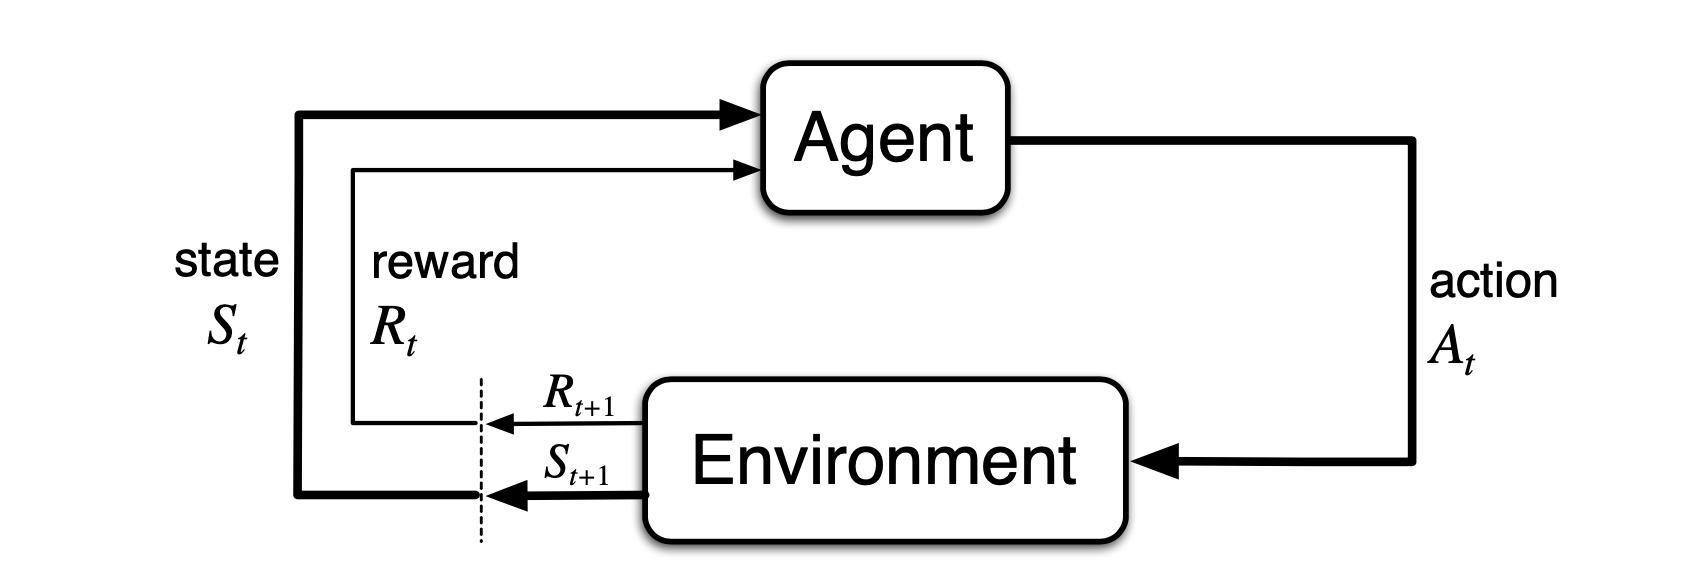
\includegraphics[width=0.8\linewidth]{img/mdp.png}
\caption{Agent-environment interactions in a MDP}
\end{center}
\end{figure}

\paragraph{} The agent and the environment will interact at each sequence of time t = 0,1,2,3,4,... At each timestep t, the agent receives a state $S_t$ and will offer an action $A_t$ from what he knows. Then, the environment, as a result of this action, will return a reward $R_t$ to this action and lead the agent to a new state $S_{t+1}$. \\
It leads to a trajectory like this : 
\[ S_0, A_0,  R_1, S_1, A_1, R_2, S_2, A_2, ... \]
In our problem, a timestep corresponds to a content that is consumed (for instance a video or a music).

	\subsubsection{Returns, policy and value function}

So far we have defined our problem in term of MDPs, but we haven't defined yet the objective of the learner. 

\paragraph{Return} This is the cumulative sum of the rewards from step t. It is defined as follow : 
\[
G_t =  R_{t+1} + R_{t+2} + ... + R_{T} 
\] where T denotes the timestep where the simulation ends (the user has left the simulation for instance). \\
\paragraph{Expected return} The previous formulation of the return doesn't take into account the fact that a future actions can have an impact to the given suggestion. To cope with it, we add a \textbf{discount} factor $\gamma$ with $0 \le \gamma \le 1$. The expected reward is then defined as : 
\[  G_t = R_{t+1} + \gamma R_{t+2} + \gamma^ 2 R_{t+3} + ... + \gamma^{T-1} R_{T} = \sum_{k=0}^{T}\gamma^k R_{t+k+1}            \]
The discount factor $\gamma$ represents the value of future rewards : $\gamma = 0$ means the agent is 'myopic' and only considers maximizing current rewards whereas if $\gamma$ is close to 1, the agent takes into account future rewards. 


\paragraph{Policy } Mapping from states to probabilities of selecting an action. If an agent is following a policy $\pi$ at time t, then $\pi(a|s)$ gives the probability of choosing the action $A_t = a$ from state $S_t = s$.

\paragraph{Value function} The value function of a state s under a policy $\pi$, denoted as $v_{\pi}(s)$ is defined as the expected return when starting from the state s and following the policy $\pi$ :  
\[ 
v_{\pi}(s) = E_{\pi}(G_t | S_t = s) 
\]
\paragraph{Action-value function} As described above, we define the value of taking action a in state s under a policy $\pi$, denoted $q_{\pi}(s,a) $, as the expected return from state s, taking the action a and following the policy $\pi$ : 
\[ q_{\pi}(s,a) = E_{\pi}(G_t | S_t = s, A_t = a) \] 


\section{Q-Learning}

\subsection{Optimality}

\paragraph{} There are different policies that can handle a reinforcement learning problem. Nevertheless, some policies are better than others. But what does better mean in MDP ? 
\paragraph{Order in term of policy} A policy $\pi$ is better than a policy $\pi'$ if its expected return is greater than or equal to that of $\pi'$ for each state.
\paragraph{Optimal policy} There is always at least one policy which is greater than or equal to every other policies. Same idea for the action-value function. We denote them as follow : 
\[    v_{*}(s) = \max_{\pi} v_{\pi}(s)          \] and 
\[    q_{*}(s,a) = \max_{\pi} q_{\pi}(s,a)          \] 


\subsection{Bellman optimality equations}

The Bellman equations express the relationships between the value of a state and the value of the next states. 
Furthermore, the Bellman optimality equations express the fact that the value of a state under an optimal policy should be equal to the expected return for the best action from that state : 
\[  v_{*}(s)  = \max_{a} q_{\pi_{*}}(s,a)   = \max_{a} \sum_{s',r} p(s',r | s,a) [r + \gamma v_{*}(s')]                \]
There is the equivalent equation for the state action value function : 
\[  q_{*}(s,a) = \sum_{s', r} p(s',r |s,a) (r + \gamma \max_{a'} q_{\pi}(s',a')    )        \]
This is actually a system of equations for each state. \\
Once the optimal function of state-action pairs is determined, one can infer the optimal action to take from a given state s  : 
\[   argmax_{a'} q_{*}(s,a')                \]
Therefore, after determination of the optimal Q-table, we know which content to recommend for the user for each content in the catalogue.

\subsection{Q learning algorithm}
\paragraph{} To learn how to approximate the optimal state action pairs, we can approximate directly $q_{*}$. To do so, we use this following formula : 

\[   Q_{t+1}(S_t, A_t) =   Q_{t}(S_t, A_t) + \alpha (R_{t+1} + \gamma \max_{a} Q(S_{t+1} , a) - Q_{t}(S_t, A_t)        )            \]

It leads to the Q learning algorithm : 

\begin{figure}[h!]
\begin{center}
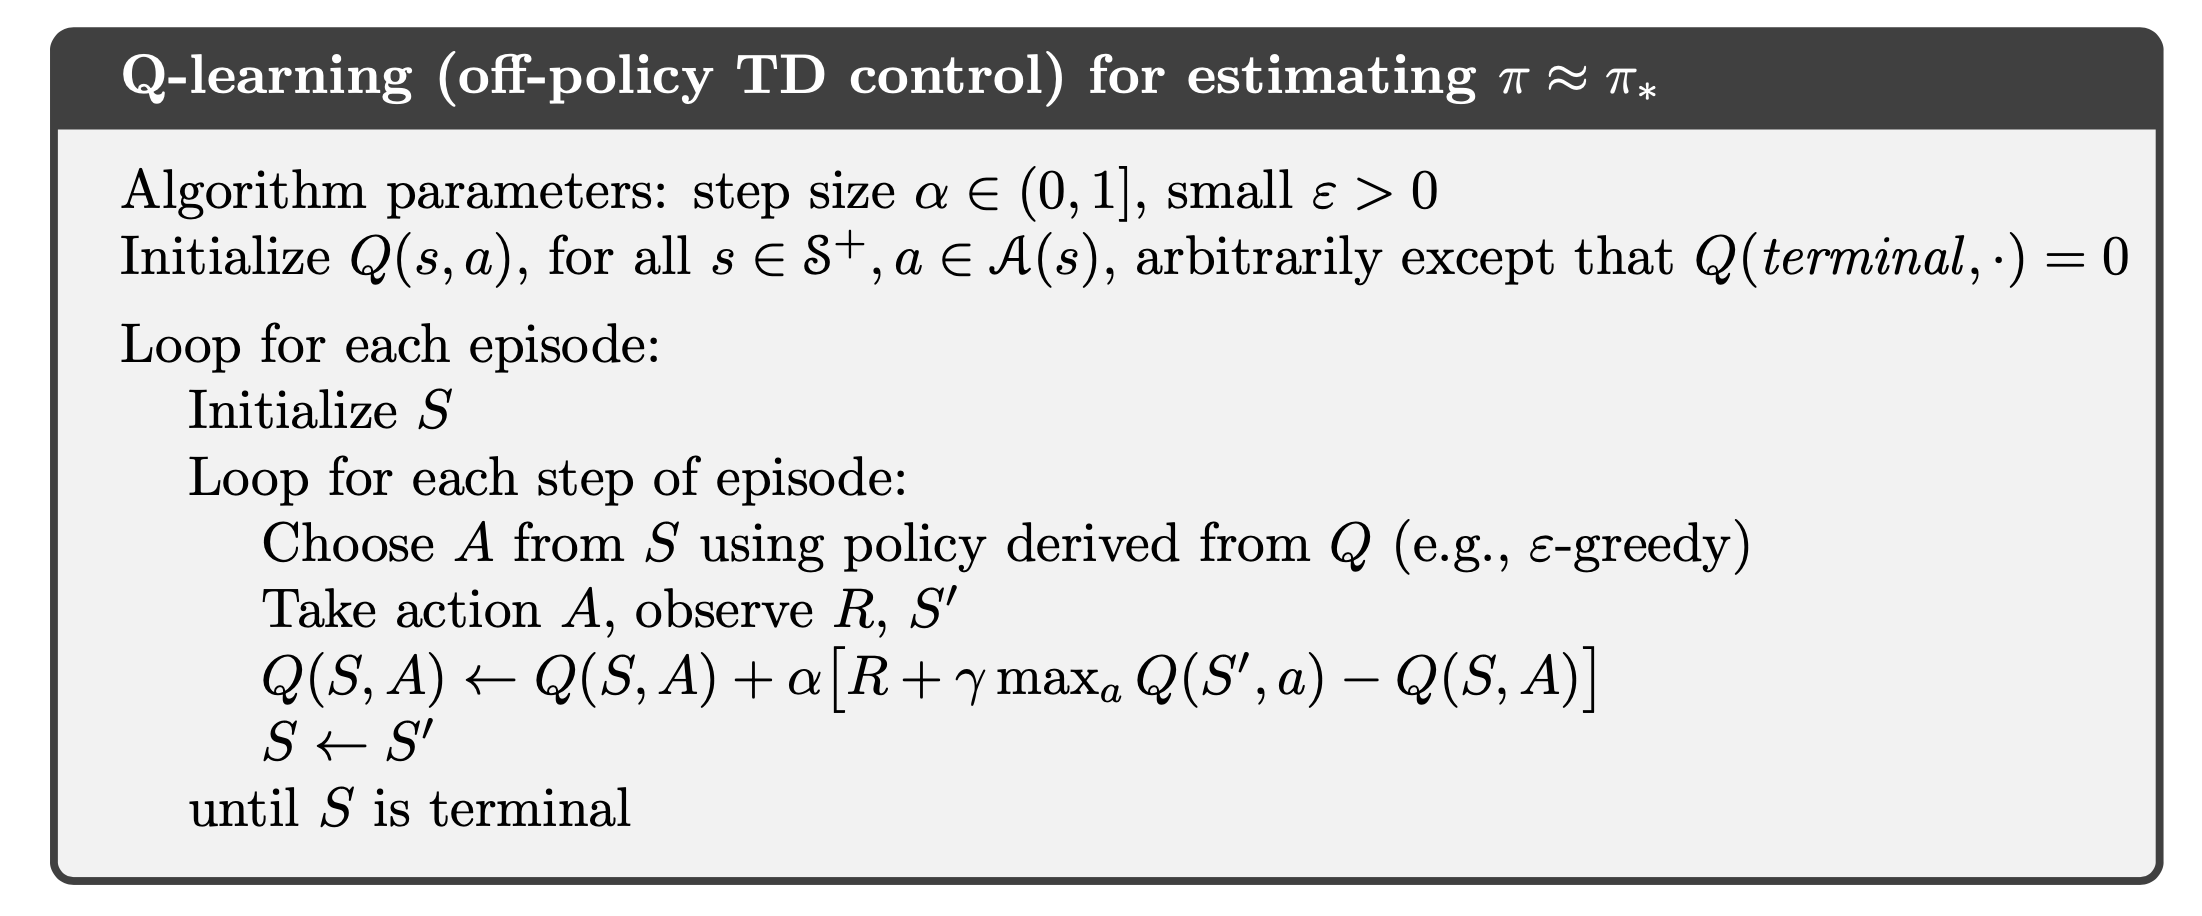
\includegraphics[width=1.2\linewidth]{img/qlearning.png}
\caption{Q learning algorithm}
\end{center}
\end{figure}

\newpage

\subsection{Exploration and Exploitation ($\epsilon$-greedy)}


In the above algorithm, the selection of an action by the agent (and so the content to recommend) is chosen in a specific way. Indeed, there is a trade-off between : 
	\begin{enumerate}
		\item \textbf{Exploration} : with probability $\epsilon$, the agent will pick randomly a content among the catalogue. The purpose is to enable the agent to continue to explore the possible actions in order not to avoid some good decisions.  
		\item \textbf{Exploitation} : with probability $1 - \epsilon$, the agent will pick the action that maximises the q-values : $argmax_{a}  Q(S_t, a)   $
	\end{enumerate}
This is very important to keep this trade-off : avoiding the exploitation will lead to random recommendations whereas avoiding the exploration will lead to eventually bypass good actions. \\
Furthermore, one can consider to start with a high $\epsilon$ to advantage the exploration (because we have no knowledge of the expected rewards yet) and then gradually decreasing the $\epsilon$ as the agent learns more and more about the environment.\\
 Nevertheless, we don't consider this approach because it is equivalent to assume that the user doesn't change and he keeps his preferences. We don't consider that configuration and we keep $\epsilon$ constant.  
    
    
\subsection{Convergence criteria}
There are two ways to consider the end of the algorithm, and therefore to get the final Q values (which should correspond to the optimal Q-values) : 
	\begin{enumerate}
		\item \textbf{Number of epochs} : We simulate user experiences and in the same time we update the Q-table for a number of times predefined. Then, we risk to have situation where the Q-table values don't update anymore and we compute for nothing.
		\item \textbf{Threshold} : We use a criteria to say whether the Q-table values have converged. To do so, we consider the maximum difference of Q-table values over an episode. That is to say, we let the user consume contents, and whenever he has terminated, we take the maximum difference between the previous Q-table and the new one obtained after the simulation. If this value is less than a threshold (new hyperparameter), then we stop the process and we consider the Q-table as optimal.
	\end{enumerate}
    
    
 \subsection{Hyperparameters}
 There are some hyperparameters to take into account in the Q-learning algorithm. 
 \begin{enumerate}
 	
	\item \textbf{Learning rate } $\alpha$ : it describes how fast we want to adjust the  Q-values. This is as a classic supervised algorithm with gradient descent : a too high value of $\alpha$ leads to divergence whereas a too low value leads to increase the convergence time. 
 	\item \textbf{Discounted } $\gamma$ : It deals with the rewards that the agent considers to update the Q-values. Indeed, if $\gamma = 0$ the agent will prefer actions with high current rewards whereas $\gamma$ close to 1 will lead the agent to consider actions that lead to future high rewards. For instance, if $\gamma = 0.9$, it will take into account 10 future episodes.
	
 \end{enumerate}
 
 	Furthermore, there are also hyperparameters for the environment (and so the user we use). If the user is a Markovian one, the hyperparameters are the following : 
	
	\begin{enumerate}
	
	\item \textbf{Cached contents} : Number of cached contents. This is what takes into account the network : the cached contents shouldn't cost anything to the user in order to consume it. On the other hand, a non-cached content can, if this is a popular one, lead to latency and decrease the user's experience.
	\item \textbf{Related contents} : Number of related contents for each state. For instance, if the catalogue is a list of music, the related contents can be musics from same genre or artist. We keep this number constant for each state, and it shouldn't be more than 10  percent of the total size of the catalogue (to be realistic).
	\item $\mathbf{\alpha}$ : Probability to leave the experience. It corresponds to the end of a user experience. For instance, it could correspond to the time spent on Youtube watching consecutive videos.
	\item \textbf{a} : Probability that the user follows our recommendations. This coefficient is set constant for sake of simplicity, but should evolve through the process. Indeed, if we recommend contents that the user dislikes, he won't trust the recommender and so will choose himself the future contents. We consider this factor as stationary : it doesn't evolve through the experience.
	\end{enumerate}
	Note that for the specific user described above, the only difference is in the a coefficient. 


\subsection{Results}

	\subsubsection{Q-table}
	
	We tried to solve two different problems : 
		\begin{enumerate}
			
			\item \textbf{Classic recommender} : In the exploration part, we consider all the contents with uniform probability.
			\item \textbf{Restricted recommender} : In the exploration part, we only consider the related contents (we use the non null values in the U matrix and don't suggest the others).
			
		\end{enumerate}
	Hence, we expect different behaviours for the final q-tables.  \\
	Note that we have also generated an environment where the catalogue has a size of 50. The cached contents are the contents 6, 13, 23, 35 and 46.\\
	We also consider that a content that is related and cached will lead to a reward of +2, whereas a content that is either related or cached will lead to a reward of +1. Finally, a content neither related nor cached will lead to a reward of 0. \\
	Here are the results of a q-table after applying the Q-learning algorithm for 100 000 epochs :
	\begin{figure}[h!]
    \centering
    \subfloat[Classic recommender ]{{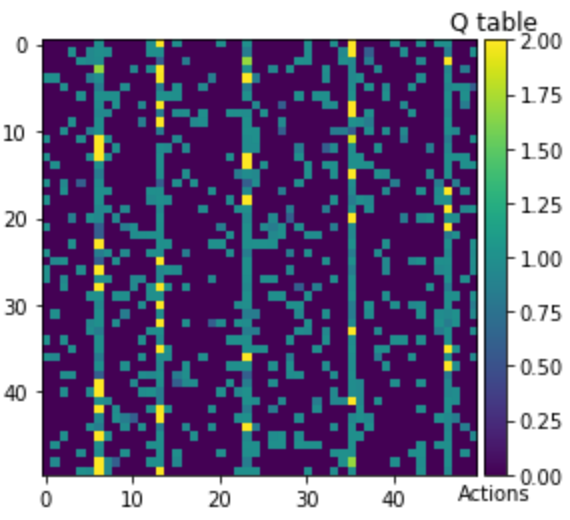
\includegraphics[width=5cm]{img/gamma0_no_c.png} }}%
    \qquad
    \subfloat[Restricted recommender]{{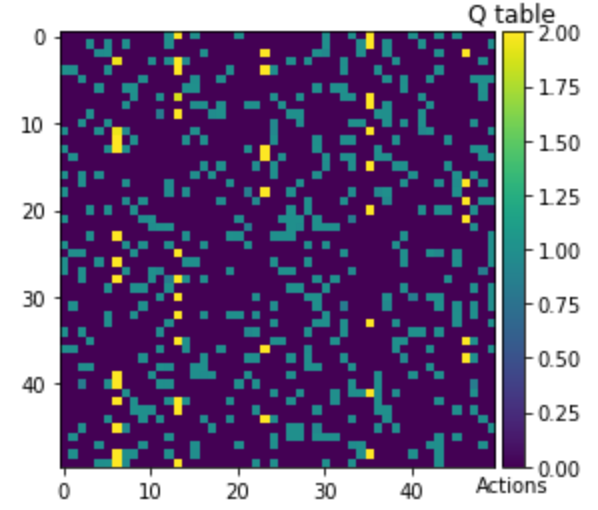
\includegraphics[width=5cm]{img/gamma0_c.png} }}%
    \caption{Q-tables for $\gamma = 0$ }%
    \label{fig:example}%
    \end{figure}
	
	
	
\paragraph{}	To understand what these plots mean, it requires to read it line by line. In fact, for a given state (a line in these plots), the values we got in this line are the expected rewards for recommending this action (content). We can see that, as the cached contents are fixed, the vertical lines correspond to these contents. Moreover, whenever a q-value is yellow (which means the q value associated is very high), the content is related and cached. \\
\paragraph{} The difference between a classic recommender and the restricted one is that the restricted recommender tends to not consider every content in the catalogue. It leads, as shown above, to make the q-table values to 0 for contents that are cached (because they are not related to the specific state).
	 
	
	\subsubsection{Discounted $\gamma$ parameter}
	\paragraph{} To understand the role of $\gamma$, we can focus on the optimal Q-table obtained for extreme values of $\gamma$.
	The result is shown on Figure 4, with the same environment defined above.
	
    \begin{figure}[h!]
        \centering
        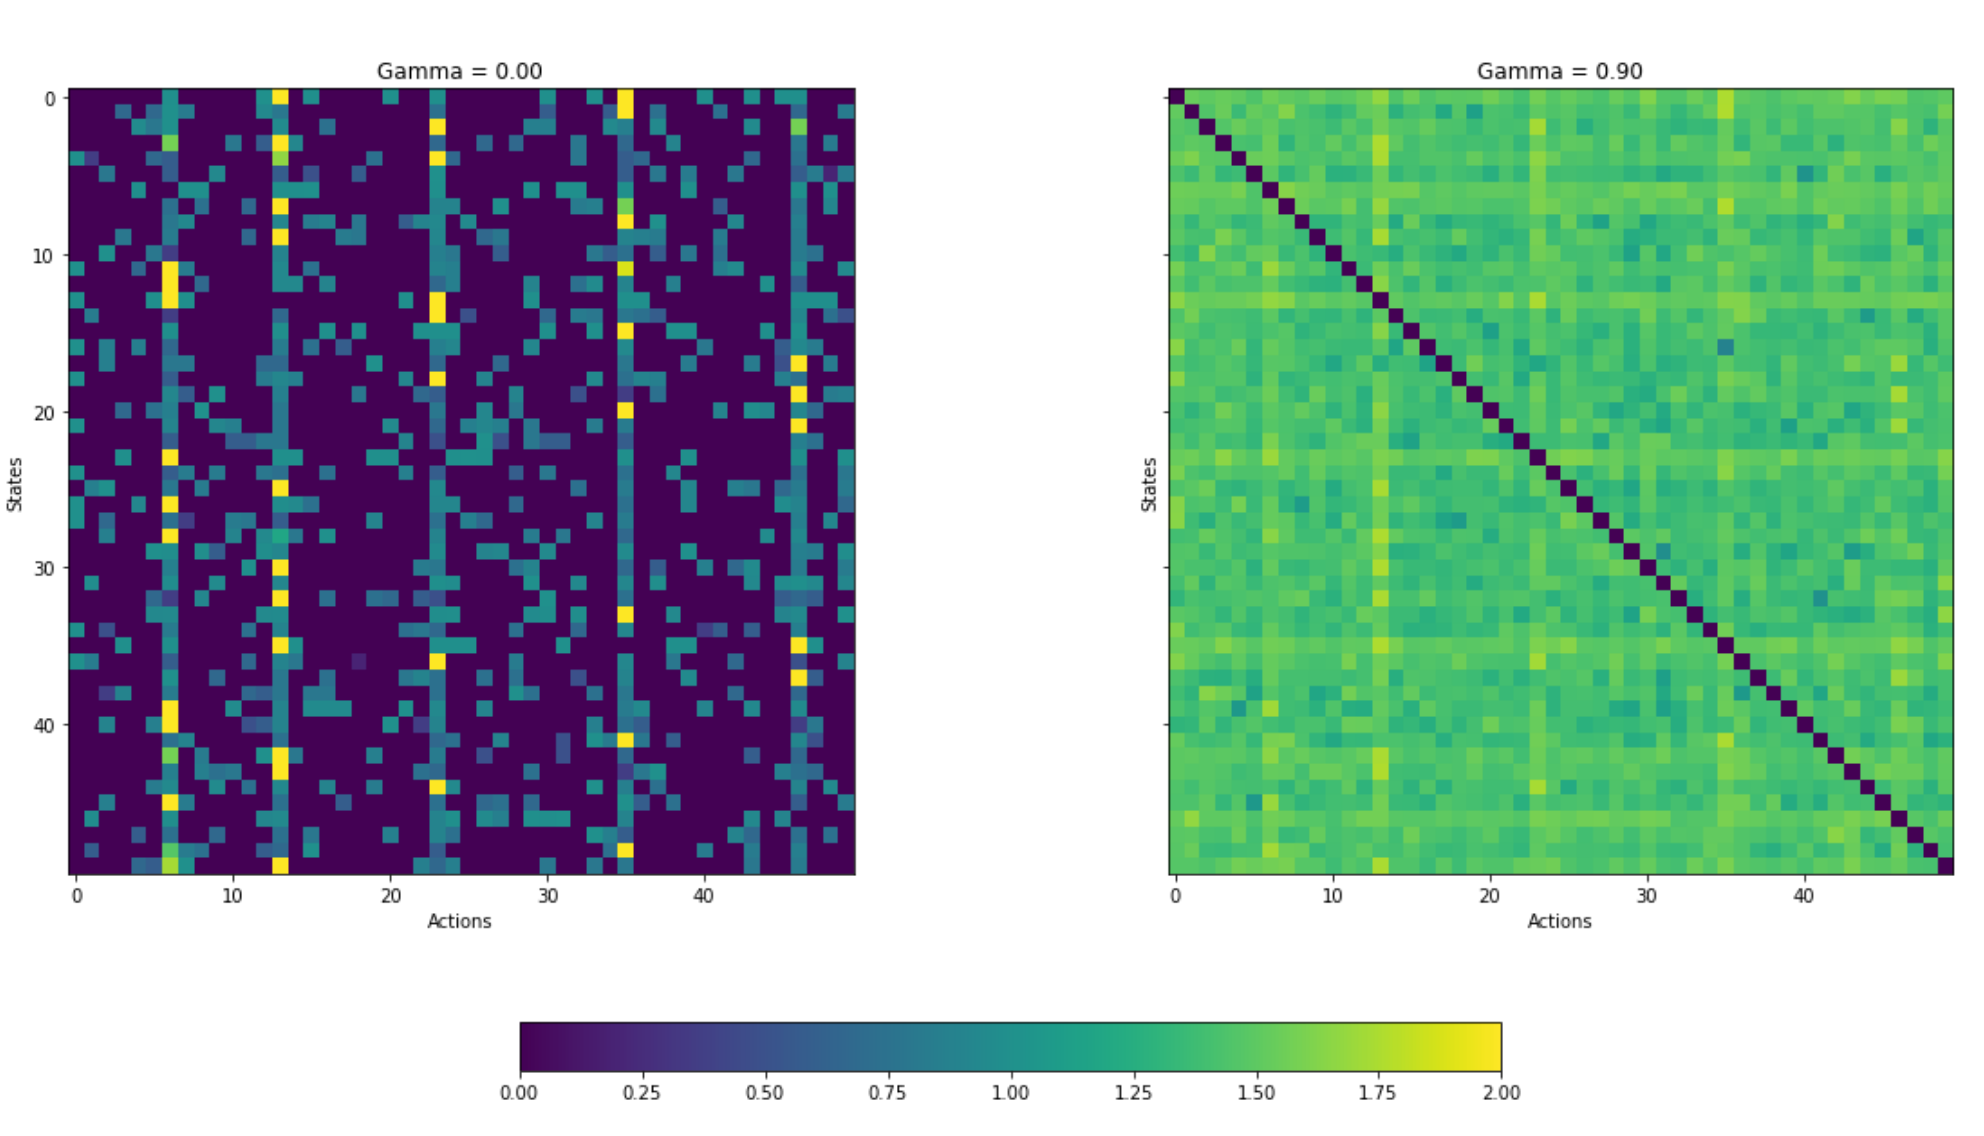
\includegraphics[scale = 0.3]{img/gamma_no_constraints.png}
        \caption{Q-table for $\gamma = 0$ (left) and $\gamma = 0.9$ (right) without constraints on the recommendations}
        \label{fig:my_label}
    \end{figure}
	
	\paragraph{} On one hand, the q-table for $\gamma = 0 $ is predictable. This can be found with both the U matrix and the cached list. Indeed, it only considers immediate rewards, which is directly linked to the fact that a content is either related or cached.  \\
	On the other hand, for $\gamma = 0.9$, we see that this is more noisy. The Q-table values are very close. As it considers future rewards, even a not cached and not related content can lead to high rewards. That's why the values are so close. The diagonal is equal to 0 because we can't recommend the content that the user is currently consuming.\\
	 
	 \newpage
	 
	 
	 
	\subsubsection{Rewards and penalties}
	\paragraph{Rewards} As the agent starts without any knowledge on the user, he will start by recommending bad actions (contents that will lead to low rewards). Through the epochs, the Q-table will start to be completed and then the agent will be able to recommend good contents. It means that, if we look at the rewards, it will start to be very low (because the agent recommends bad contents) and will progressively increase. 
	
	\paragraph{Penalties} We can also consider the quality of each decision of the agent. To do so, we consider what we call the \textit{penalty}. This value is increased each time the agent recommend a content neither related nor cached (a content that leads to a reward of 0). In this case, we expect the penalty to be the contrary of the rewards : it will start very high because the user won't know anything about the environment, and then start to learn and so the penalty will decrease. 
	\paragraph{}	Note that for both the penalties and the rewards, we take the running mean to plot it because these values are very noisy (due to the fact that the user doesn't listen to the agent every time and also due to the exploration part).
	
		\begin{figure}[h!]
    \centering
    \subfloat[Rewards]{{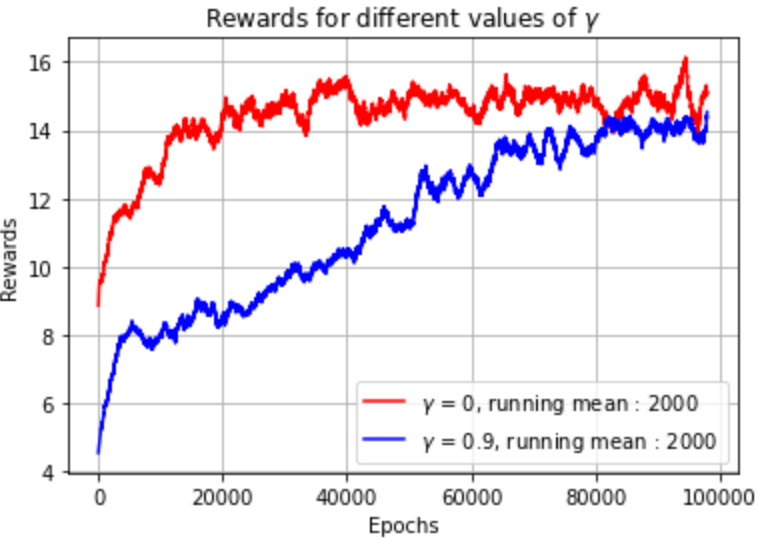
\includegraphics[width=5cm]{img/rewards.png} }}%
    \qquad
    \subfloat[Penalties]{{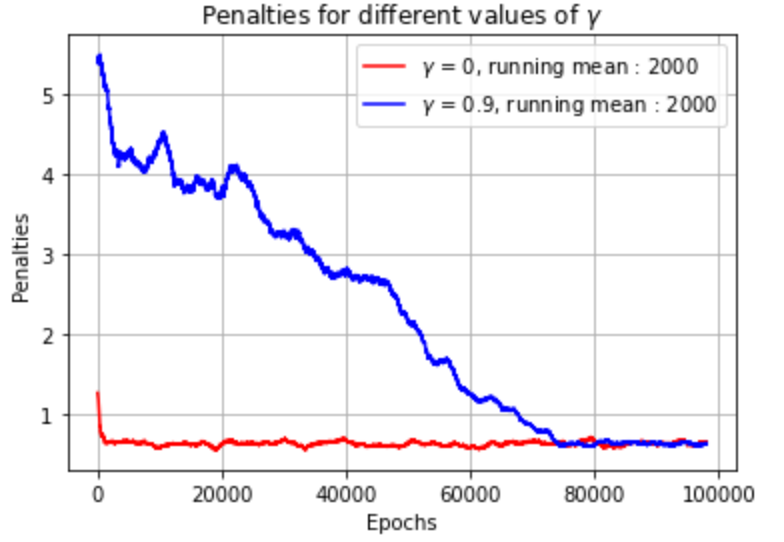
\includegraphics[width=5cm]{img/penalties.png} }}%
    \caption{Rewards and penalties for $\gamma = 0$ and $\gamma = 0.9$ without restrictions on recommendation }%
    \label{fig:example}%
    \end{figure}
	
 \paragraph{} We used different values of $\gamma$ for the plots. In fact, when $\gamma = 0$, the solution is easier to find compared to high values of $\gamma$ (because it should consider future rewards and not immediate rewards). We see that, in average, after convergence, the agent suggests contents such as the total reward per episode is around 15 (the user is consuming in average 10 contents). Furthermore, for $\gamma = 0.9$, the agent starts by suggesting 5 contents that are neither related nor cached in a session of 10 contents in average. The start is really bad but it converges to a penalty of 0 (which means no bad contents recommended).
 
 \subsubsection{Specific user}
 We've tried to simulate a Markovian user, who listens to us with some probability, otherwise he picks randomly a content among the catalogue. 
 There is another specific user that we tried to learn from. This is the user that accepts the content $j$ from the state $i$ with probability $a_{i,j} = \frac{u_{i,j}}{max_i (u_i)}$. This user is made to compare the policy to an optimization solution. The environment is composed of a catalogue of size 30, and there is only the 3 first contents that are cached. In the optimization algorithm, the process was run in 100 episode in average, which corresponds in our case to $\gamma = 0.99$. \\
 We got 28 out of 30 contents that are similar in terms of policy : 
 
 \begin{figure}[h!]
     \centering
     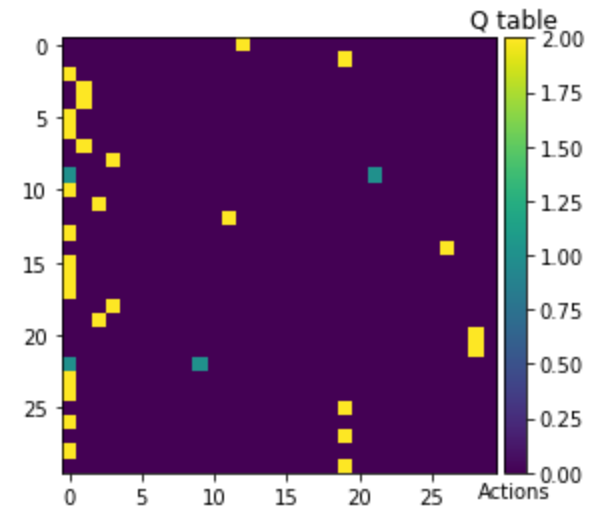
\includegraphics[scale = 0.6]{img/specific_user.png}
     \caption{Sum of the optimised policy and our policy with constraints with Q-learning algorithm}
     \label{fig:my_label}
 \end{figure} 
 
 In this plot, we represent the sum of our policy for the given user and the policy after application of the optimised algorithm. It tells us the final content to recommend when the user is consuming a specific content (so for each line). Each time the plot above has value equal to 2 (in yellow), it means both our algorithm and the optimised algorithm has predicted the same action for the given content that the user is consuming. On the other hand, if the value is 1 (and therefore there are two values equal to 1 for this line), it means the algorithms will recommend something different (which happens 2 times out of 30). It means our algorithm has similarity with a classic optimized approach.
 
 
 
\subsubsection{Time of convergence}

    \paragraph{Criteria of convergence} As explained above, the criteria to say whether the agent has finished to learn or not is either a maximum number of episode or the maximum difference between q-tables over an episode. The last criteria should decrease when the epochs increase : 
    
    \begin{figure}[h!]
        \centering
        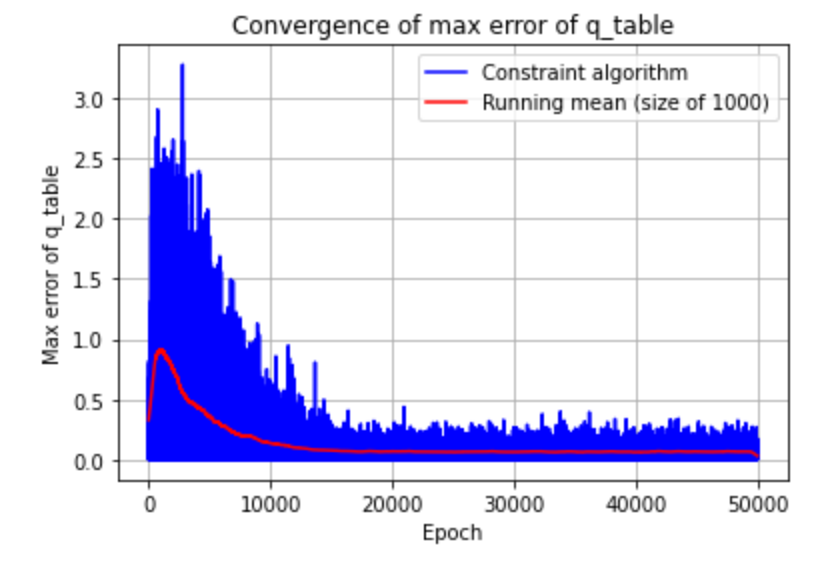
\includegraphics[scale=0.5]{img/convergence.png}
        \caption{Evolution of the maximum difference of q-table ($\gamma = 0.9$) }
        \label{fig:my_label}
    \end{figure}
    Therefore, we decided to take as a threshold 0.08.

    \paragraph{Time of convergence} What becomes interesting is the time of convergence of the algorithms. Indeed, here the catalogue size is 50. But in reality, the catalogue size can be million of contents. To have an idea of the time required, we looped over the size of the catalogue and we stored the time required to converge (for $\gamma = 0.9$). We set the size of the related contents to 5$\%$ of the catalogue size and the number of cached contents to 4 $\%$ of the catalogue size. We increased the size of the catalogue and reported the number of episodes and the time until convergence.
    
    \begin{figure}[h!]
        \centering
        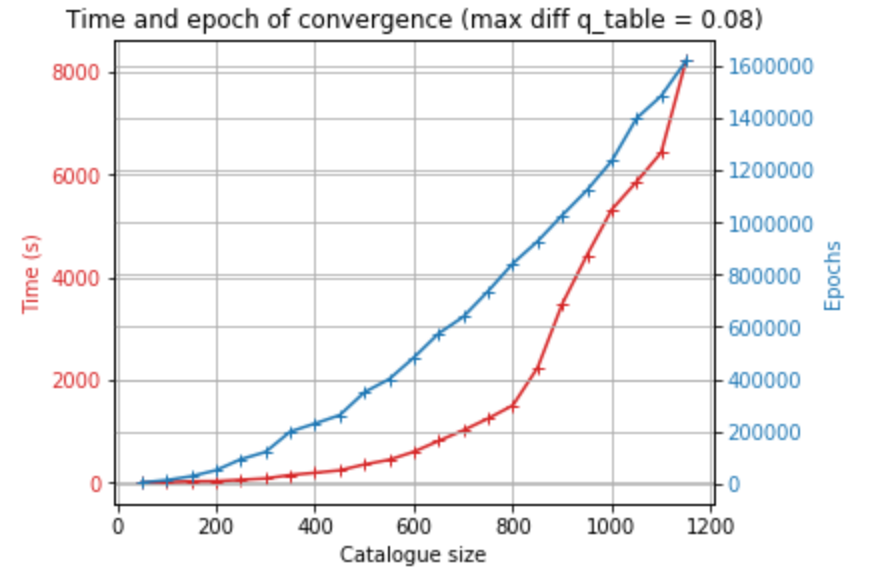
\includegraphics[scale = 0.5]{img/convergence_time_epochs.png}
        \caption{Time and epochs for convergence depending on the catalogue size}
        \label{fig:my_label}
    \end{figure}

    \paragraph{} Therefore, for a catalogue size of 1200, it took 2 hours and around 1 600 000 episodes until convergence. Furthermore, if we want it to be realistic, we need to add the time of consumption of a content by the user. Indeed, for a music, it would require 3 minutes in average, and for videos it will be even more. So, for musics, it will require 400 hours until convergence, and for only 1200 songs. 
    Thus, we need a way that requires less time to compute in order to improve the quality of the user's experience.

\section{Deep Q-learning}

\subsection{Function approximation}
\paragraph{} As we want to represent a real data set of contents, we need to have a large amount of states in the catalogue, and therefore in the Q-table too. To do so, the function approximation seems appropriate. It will use a neural network to approach the Q values. It takes as input a state and produces the Q values for every action.  The aim of the neural network is to learn the parameters that will lead to generate the Q-tables.

\begin{figure}[h!]
    \centering
    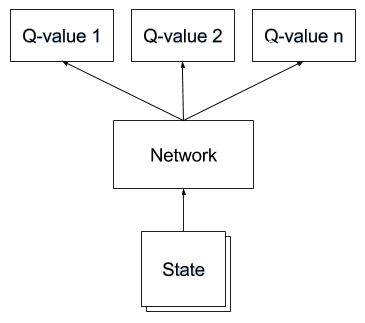
\includegraphics[scale = 0.5]{img/function_approx.png}
    \caption{Function approximation summary}
    \label{fig:my_label}
\end{figure}

We denote the new q-table as : $Q(S_t, A_t , w)$ in order to have a notation where we know that this is an approximation with neural network.


\subsection{Training part}

\paragraph{} To train the neural network, it requires a target such as in supervised learning. Indeed, the parameters of the neural network can be update thanks to the gradient of the loss according to these parameters. \\



\paragraph{Target} What we want to approximate is the Q-table, that is to say the expected rewards from a state for each action available. Therefore, as for the Q-learning algorithm, the target is the following : 
\[  R(S_t, A_t) + \gamma \max_{a} Q(S_{t+1}, a, w)              \]
At the beginning of the training, the next maximum reward predicted by the model will be wrong (the model isn't trained yet). The only thing that is sure is the actual reward $R_t$, which should slowly adjust the network parameters.

\paragraph{Loss} To update the weights, we need a loss. As the problem is a regression problem, we can use the Mean Square Error between the target and the actual output of our network. It gives the following formula : 
\[  loss = (R(S_t, A_t) + \gamma \max_{a} Q(S_{t+1}, a, w) - Q(S_t, A_t , w))^2                                  \]
Note that the Q-table for the prediction of the target and for the actual prediction is the same. A different version exists, where we use two different neurons : one for the target and one for the actual prediction. This is the double Q-learning algorithm. 

\paragraph{Memory replay} To build a batch that isn't correlated, what is usually done is the experience replay (or memory replay). This is done by storing each experience (which corresponds to an episode) : the State, Action, Reward, Next state and if the experience ended after this or not. In our case, if the experience had ended it was because the user left the experience. The memory replay will be used during the training : instead of updating the network for each episode of the user, we use a mini-batch where we extract experiences from the memory replay.

\begin{figure}[h!]
    \centering
    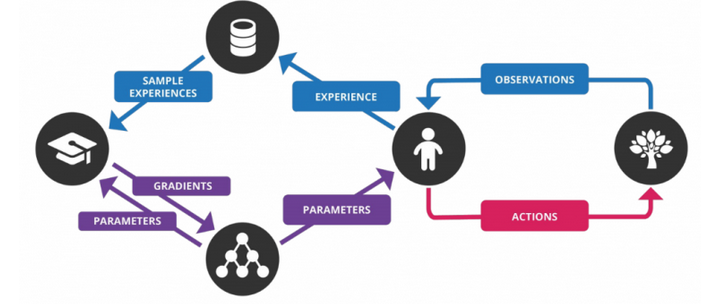
\includegraphics[scale = 0.5]{img/schema-dq.png}
    \caption{Summary of deep Q-learning for reinforcement learning}
    \label{fig:my_label}
\end{figure}


\subsection{State representation}

\paragraph{} For the classic Q-learning algorithm, we represent a content as a number. For instance, the content 15 was represented by the integer '15'. Nevertheless, we can't do this anymore. Indeed, if we were to use this representation, the neural network would make the same amount of epochs than the Q-learning algorithm to converge. The aim of using function approximation is to let the neural network approximate the states, and therefore to find similarities between states that are 'close' in terms of actions to suggest. To do so, we need to change the representation of the states. 

\paragraph{One hot encoding }
For a given state $S_t = i$, we replace this state by a list of contents where there is 0 everywhere except for the i position :
\[\Phi(S_t = i ) = [ 0, ... , 1, ... 0         ]   \]

\paragraph{U matrix }
For the state $S_t = i$, we replace this state by the corresponding line of the U matrix : 
\[   \Phi(S_t = i ) = u_i  \]
As the U matrix has values (corresponding to similarity between two contents) between 0 and 1, the algorithm would have to learn that a content that has U values equal to 0.88 or 0.76 will lead to same rewards. So another way to represent it better would be to make 1 whenever the U values isn't null and 0 otherwise : 
\[ \Phi(S_t = i ) = (\delta_{i,j})_{1 \le j \le n  } \text{ where } \delta_{i,j}
\begin{cases}
    1& \text{if } u_{i,j} \ne 0   \\
    0             & \text{otherwise}
\end{cases} \] 

\paragraph{Rewards}
For the state $S_t = i$, we replace by a list of contents where there is 0 if the content is neither related nor cached, +1 if it is either related or cached and +2 if the content is both related and cached : 
\[ \Phi(S_t = i ) = (\delta_{i,j})_{1 \le j \le n  } \text{ where } \delta_{i,j} 
\begin{cases}
    2& \text{if j is cached and related}   \\
    1 & \text{if j is cached and not related or related and not cached} \\
    0 & \text{otherwise} 
\end{cases}  \]


\paragraph{Valuable } Finally, to help even more the algorithm to find the Q-table values, we can try to add information about what the following action would lead to. We replace the state $S_t = i$ by $\delta_{i,j}$ where : 
\begin{enumerate}
    \item $\delta_{i,j} = 0$ if $u_{i,j} = 0, x_j = 1, \forall k \in [1,K], u_{j,k} \ne 0 \land x_k = 1   $
    \item $\delta_{i,j} \mathrel{+}= 1$ if $u_{i,j} \ne 0$
    \item $\delta_{i,j} += 1$ if $x_j = 0$
    \item $\delta_{i,j} += 1$ if $\exists k \in [1,K], u_{j,k} \ne 0 \land x_k = 0 $
\end{enumerate}
In other words, we replace the state by actions where we add 1 whenever the action is either cached, related, or if the next state it leads to has at least one related content that is cached.

\paragraph{}
To visualise the previous representations, Figure 11 is a plot of the representation. For each line of these matrices there is the new representation of the given state.
	\begin{figure}[h!]
    \centering
    \subfloat[One hot encoding]{{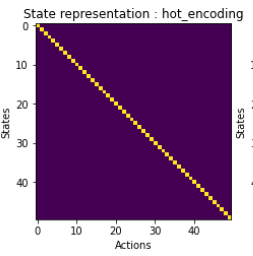
\includegraphics[width=5cm]{img/states_rep_one_hot.png} }}%
    \qquad
    \subfloat[Rewards]{{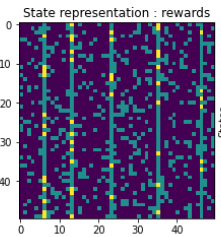
\includegraphics[width=5cm]{img/states_rep_rew.png} }}%
    \qquad
    \subfloat[U matrix]{{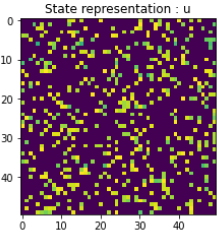
\includegraphics[width=5cm]{img/states_rep_u.png} }}%
    \qquad
    \subfloat[U one hot encoded matrix]{{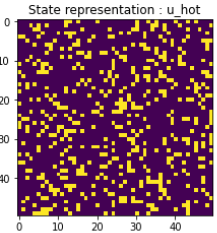
\includegraphics[width=5cm]{img/states_rep_u_hot.png} }}%
    \qquad
    \subfloat[Valuable]{{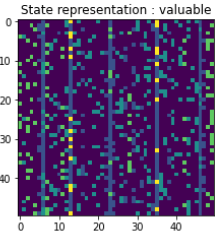
\includegraphics[width=5cm]{img/states_rep_valuable.png} }}%
    \caption{Different state representations for deep q learning algorithm }%
    \label{fig:example}%
    \end{figure}
	
\newpage

\subsection{Algorithm}
To summarize, we used the following algorithm to get the q-table for our problem : 

\begin{figure}[h!]
    \centering
    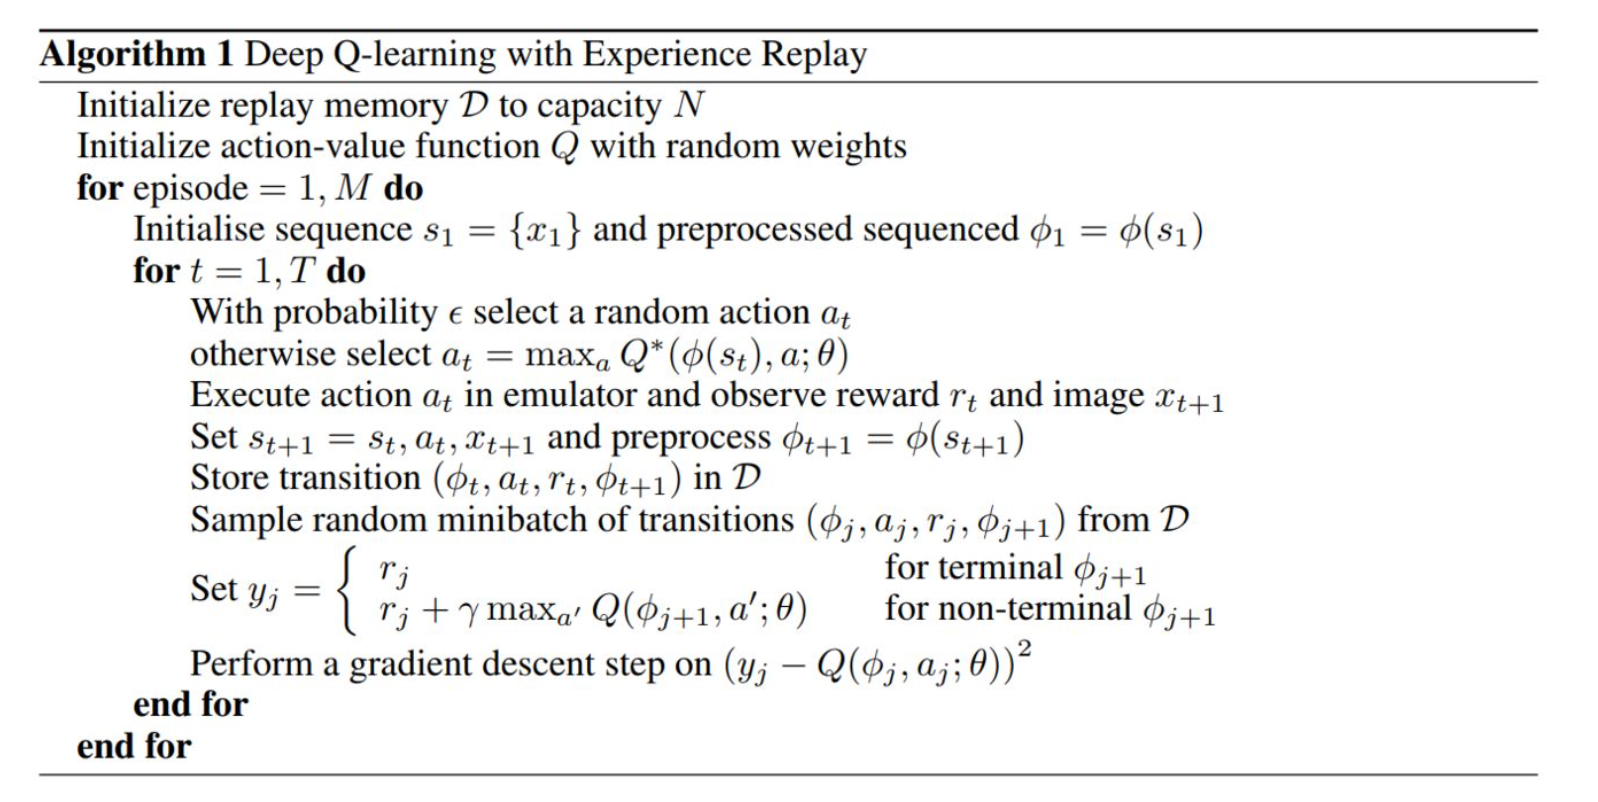
\includegraphics[scale = 0.4]{img/deep_q_algorithm.png}
    \caption{Deep Q-learning pseudo code }
    \label{fig:my_label}
\end{figure}


\subsection{Results}

    \paragraph{Environment} To compare among all the different representations, we generated one environment. The U matrix was generated randomly like the cached contents. The hyperparameters of the environment are the following : 
    \begin{enumerate}
        \item[-] Catalogue size : 50
        \item[-] Probability that the user listens to the suggestion of the agent : $a = 0.6$
        \item[-] Number of user episodes : 10 ($\alpha = 0.1$)
        \item[-] Number of related items : 10
        \item[-] Number of cached contents : 5
        \item[-] Rewards : \begin{enumerate}
            \item If the content is cached and related : +2
            \item If the content is either cached or related : +1
            \item If the content is neither cached nor related : 0
        \end{enumerate}
        
    \end{enumerate}
    
    Thus, the reward matrix (which corresponds to the immediate rewards) is the one on Figure 13 (this is the same used for the Q-learning method).
    
    \begin{figure}[h!]
        \centering
        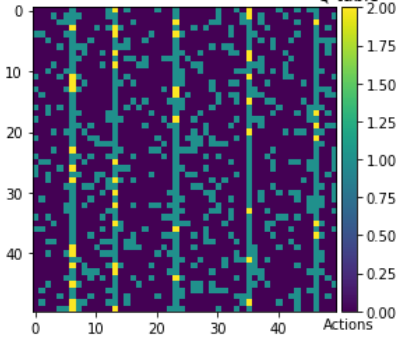
\includegraphics[scale = 0.4]{img/reward_matrix.png}
        \caption{Reward matrix}
        \label{fig:my_label}
    \end{figure}
    
    \paragraph{Q-learning results}
     We used the Q-learning algorithm to solve this problem. Note that we only consider the solution without constraints on the recommendation (even if we have implemented the constraint version). We will compare this to the deep Q-learning approach for different architecture and two different values of $\gamma$ : 0 and 0.9. 
     
    
   The results are the same shown in the Q-learning part.
    
    \begin{figure}[h!]
        \centering
        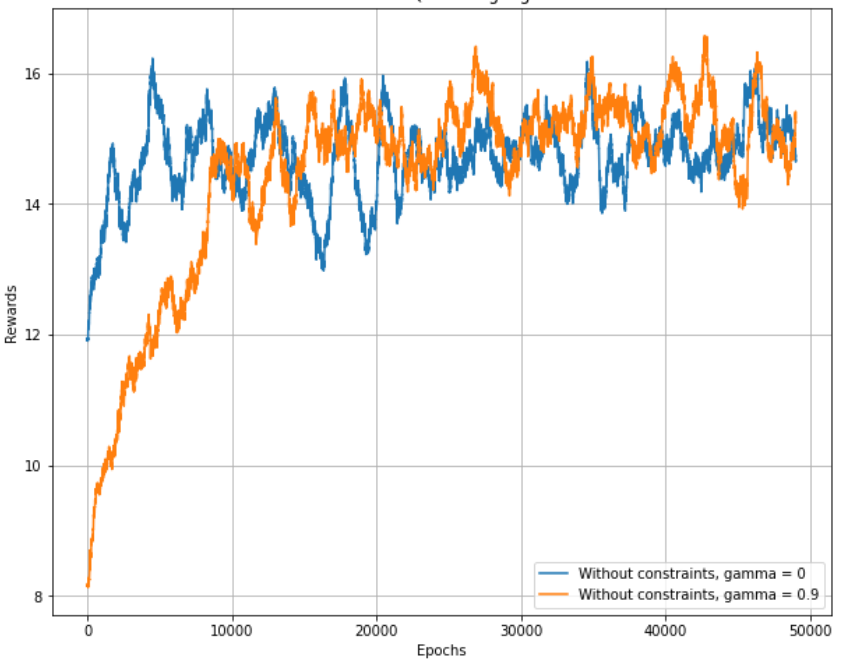
\includegraphics[scale = 0.2]{img/rewards_q_learning.png}
        \caption{Rewards with Q-learning algorithm}
        \label{fig:my_label}
    \end{figure}
    
    
    
    
    
    
    The algorithm tends to converge around 10 000 epochs, with for average a reward per episode of 15. It means that for one user experience, he will listen to 10 contents, and the agent will have for average +15 rewards (a content can have for maximum reward +2). The agent tends to recommend contents that are both related and cached, which is what is expected. A certain uncertainty remains in the algorithm as the user doesn't listen to the suggestions with a probability of $0.4$ and can leave the experience sooner that expected (with probability $0.1$). Furthermore, for $\gamma $ = 0.9, the agent can suggest contents that have bad immediate rewards if they lead to future good rewards.
    
    
    \subsubsection{Linear model}
    
        \paragraph{} To approximate our Q-table, one can consider a linear model between the features states and the Q-values.
        We used the following hyperparameters : 
        
        \begin{enumerate}
            \item[-] Memory size : 50
            \item[-] Epsilon-greedy : 0.1
            \item[-] Learning rate : 1e-4
            \item[-] Batch-size : 10
            \item[-] Optimizer : SGD
            \item[-] Number of epochs : 10 000
        \end{enumerate}
        
        \paragraph{Rewards} As we did before with the Q-learning algorithm, we stored the rewards per episode. The results are in Figure 15 : 
        
        \begin{figure}[h!]
        \centering
        \subfloat[Rewards with $\gamma$ = 0]{{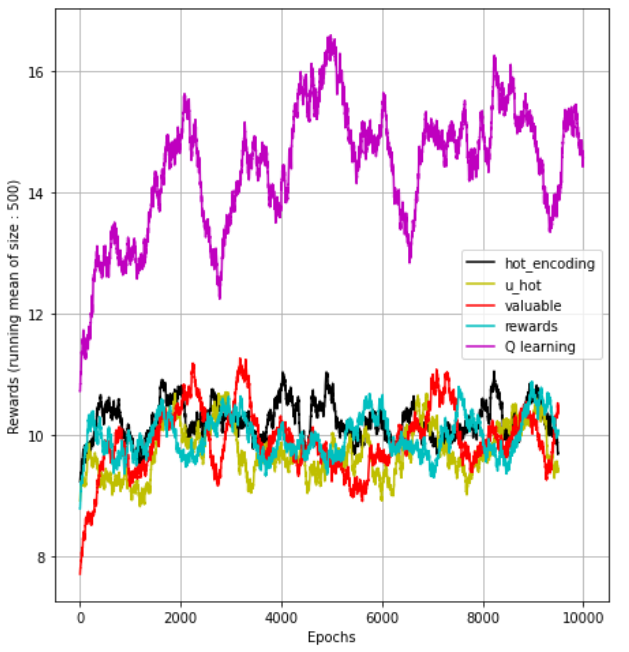
\includegraphics[width=5cm]{img/linear_0_rewards.png} }}%
        \qquad
        \subfloat[Rewards with $\gamma$ = 0.9]{{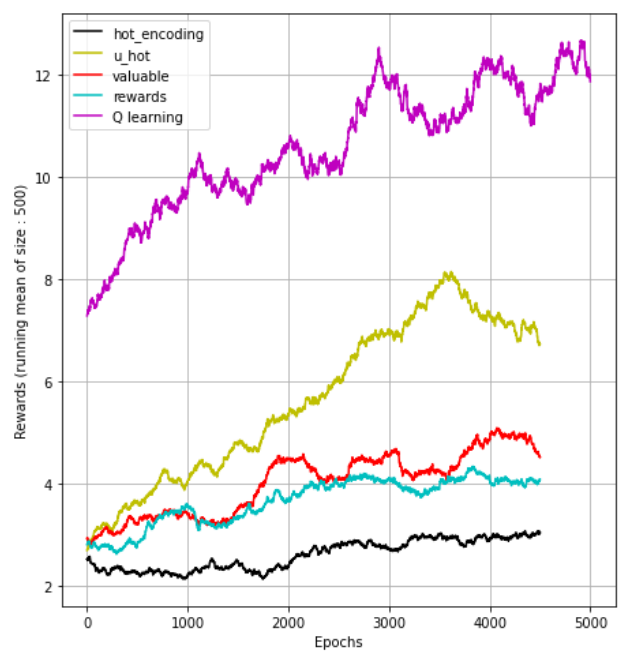
\includegraphics[width=5cm]{img/linear_09_rewards.png} }}%
        \caption{Rewards for different representation of the states and for Q-learning, for $\gamma$ = 0 (left) and $\gamma $= 0.9 (right) }%
        \label{fig:example}%
        \end{figure}

            There are few things to note here. First, the final rewards for deep Q-learning algorithm, for each representation, converge to 10 in average whereas it is 15 for Q-learning algorithm. It could be explained by the fact that for a given action, if we are in a state where this action is related, the weights will be increased whereas for another state, if the action isn't related, the weights will be decreased. \\
            Furthermore, for $\gamma$ = 0, the deep Q-learning converges much faster than the classic algorithm, which is the aim of this method. On the other hand, for $\gamma $= 0.9, the algorithm doesn't converge and doesn't do better than random suggestion. The architecture of the algorithm is maybe too simple, or it would require much more epochs to converge.

        \paragraph{Loss}
        To have an idea of how well the network learns, we can have a look to the loss defined above. The results are shown in Figure 16. 
        \newpage
        
        \begin{figure}[h!]
        \centering
        \subfloat[Loss with $\gamma$ = 0]{{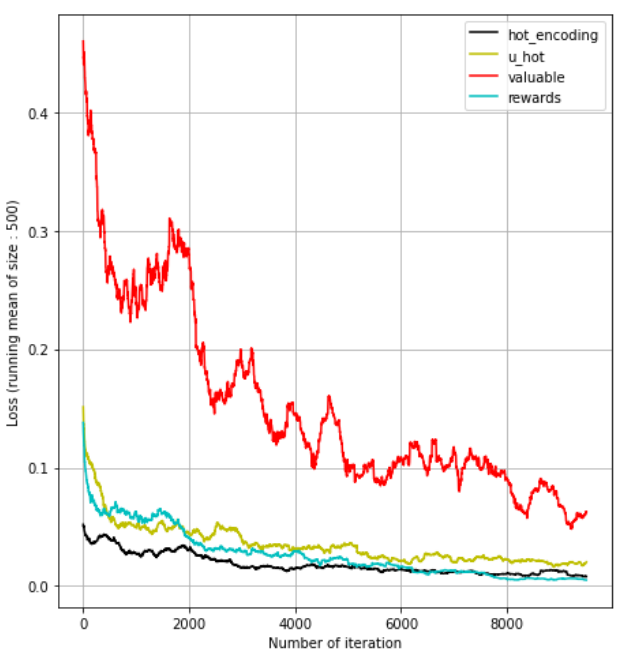
\includegraphics[width=5cm]{img/loss_linear_0.png} }}%
        \qquad
        \subfloat[Loss with $\gamma$ = 0.9]{{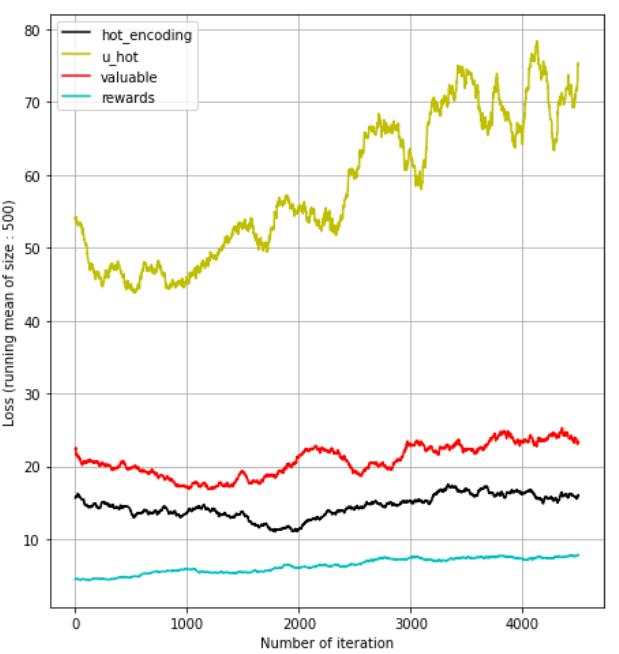
\includegraphics[width=5cm]{img/loss_linear_09.png} }}%
        \caption{Loss for different representation of the states, for $\gamma$ = 0 (left) and $\gamma $= 0.9 (right) for linear model}%
        \label{fig:example}%
        \end{figure}
        
        
        
        We see that for $\gamma $= 0, the loss is decreasing and converging. The 'one hot encoding' representation seems to be the quickest to converge whereas it is the simple representation. It could be explained by the fact that, as the solution is simple, it takes longer for a high-detailed representation to converge to a simple solution. \\
        Furthermore, for $\gamma$ = 0.9, the loss is increasing, which is related to the fact that the algorithm isn't converging. 
        
        \paragraph{Q-tables}
        After convergence, the deep Q-learning algorithm has succeeded to find the q-tables, as shown in the figure 17. 
        \begin{figure}[h!]
            \centering
            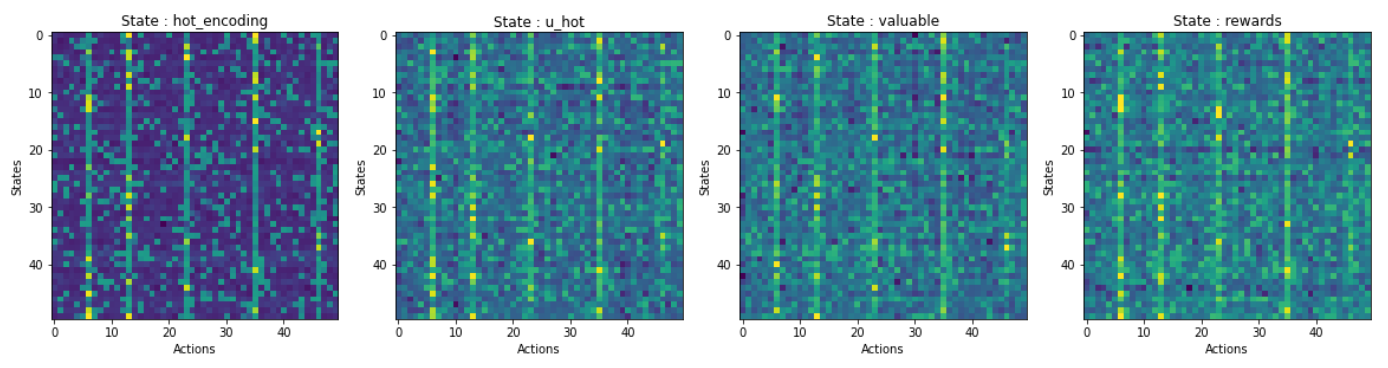
\includegraphics[scale = 0.3]{img/q_table_linear_0.png}
            \caption{Q-tables for different representation of states and $\gamma = 0$ : hot encoding, U hot encoding, valuable and rewards}
            \label{fig:my_label}
        \end{figure}
        \newline The results are very close to what we expected (for $\gamma = 0$). The algorithm has succeeded with our different representations to learn the basic solution. But it hasn't succeed in learning the most interesting part where the suggestions are not that easy. To deal with it, we can use a deeper network like with one fully connected model.
        
    \subsubsection{Fully connected model}
    \paragraph{} As mentioned above, the architecture of our network is too simple to deal with a non-trivial solution. 

            \paragraph{Architecture} We added one fully connected layer in our network of size 100. The aim is to enable the algorithm to deal by itself the complexity of the trade-off between cached and related items. 
    
        \paragraph{Rewards and loss} We tried with $\gamma$ = 0 and it works just like the linear model. We are more interesting with the results for $\gamma $ = 0.9. We can see the rewards and losses in Figure 18. 
        
        \begin{figure}[h!]
        \centering
        \subfloat[Loss]{{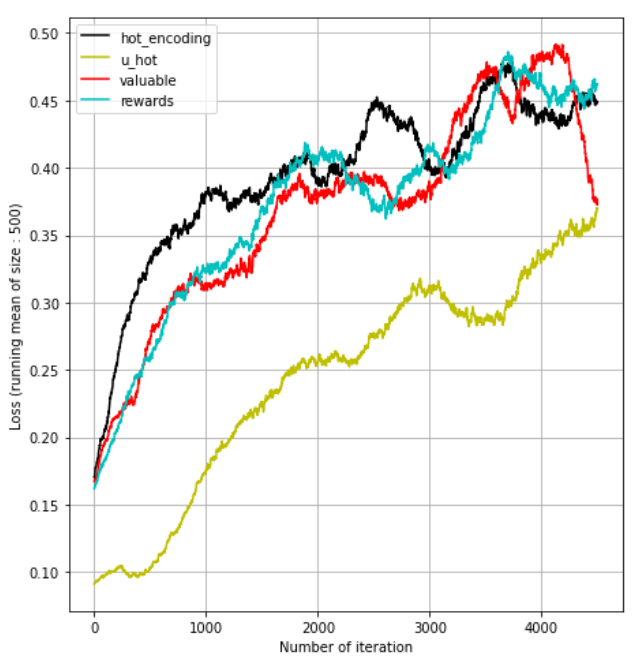
\includegraphics[width=5cm]{img/rewards_fc_09.png} }}%
        \qquad
        \subfloat[Rewards]{{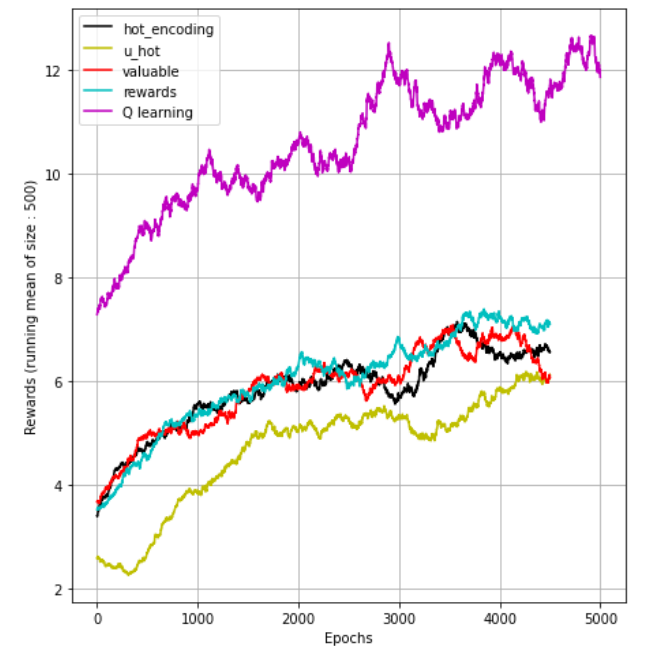
\includegraphics[width=5cm]{img/loss_fc_09.png} }}%
        \caption{Reward and Loss for different representation of the states, for $\gamma$ = 0.9 after 5 000 epochs with a fully connected model}%
        \label{fig:example}%
        \end{figure}
    
        It seems that the fully connected layer doesn't do better. We only used 5000 epochs, which can be not enough to converge as it has much more weights. The Q-learning reward is still better even if it hasn't converged yet.

        \paragraph{Q-tables} The results of the Q-tables show that it has learnt to distinguish the cached contents, but not yet the related items : 
        
            \begin{figure}[h!]
            \centering
            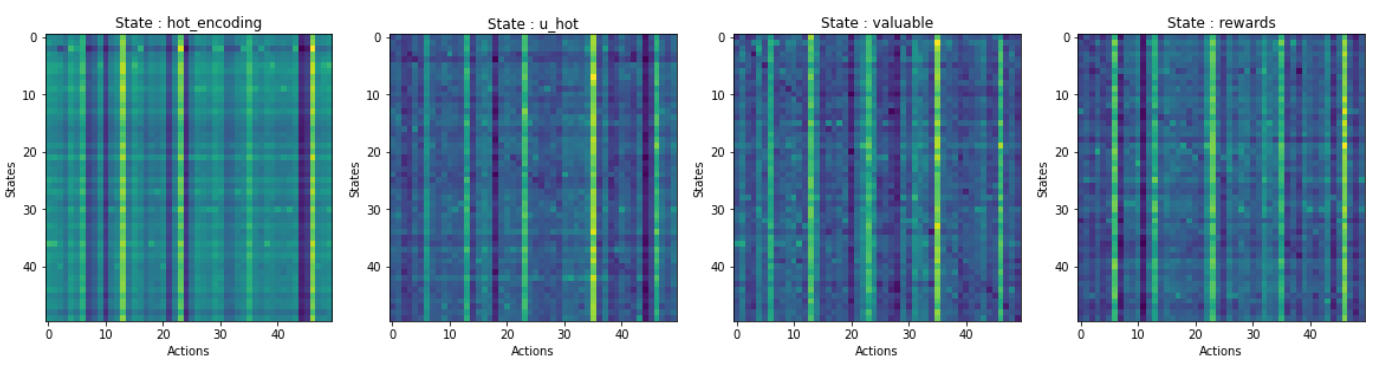
\includegraphics[scale = 0.3]{img/q_tables_fc_09.png}
            \caption{Q-tables for different representation of states and $\gamma = 0.9$ with fully connected model for : hot encoding, U hot encoding, valuable and rewards}
            \label{fig:my_label}
        \end{figure}
    Indeed, we can distinguish the vertical lines that correspond to the cached contents. But it doesn't have learnt all the related contents. 
    \paragraph{Limits} It seems that the different representations we used are too detailed. The learning part is in fact more a tabular method than an approximation. Furthermore, another thing that limits the training part (or at least make it slower) is the fact that the target and the actual prediction are computed by the same network. The target isn't fixed and leads to add even more noise.
    
\section{Double Q-learning}
\paragraph{Target network} We decided to add the fact that the target and the prediction shouldn't be from the same network. To do so, we can use a network for the target : $ (R(S_t, A_t) + \gamma \max_{a} Q'(S_{t+1}, a, w)$ and another one, that is updated at each iteration, for the prediction : $ Q(S_t , A_t,w)$. 

            \begin{figure}[h!]
            \centering
            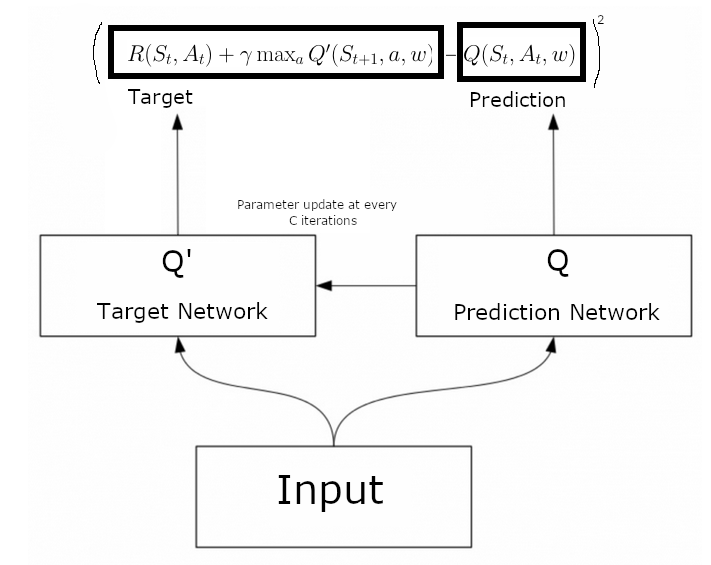
\includegraphics[scale = 0.5]{img/dqn_schema.png}
            \caption{Schema of double-Q-learning }
            \label{fig:my_label}
        \end{figure}
Then, each C iterations, the target network is loaded from the prediction network. This C value becomes therefore a hyperparameter. The aim of this method is to make the learning faster and less noisy.





\subsection{State representation} What was inferred from the previous results is that the state representations are too detailed and lead to a tabular learning. Indeed, it would require from the algorithm to test each action and then see the results to learn something, which is basically what the Q-learning does. On the other hand, if we represent the states too simply the algorithm will struggle to distinguish the related items. It requires therefore a trade-off in the representation of the states. \\
Therefore, we decided to add two new representations of the states. 
\subsubsection{Multiple} This representation is inspired by another way to code the deep Q-learning algorithm. Indeed, instead of making as input states and as output the different Q-values for each action, one could think about making as input a state and an action, which would lead the network to have a single output : the Q-value for that pair of state-action. Nevertheless, we didn't code it like that, so we decided to do things in a little different way : \\
$$  \Phi(S_t = i ) = (\delta_{i,j})_{1 \le j \le n  } \text{ where } \delta_{i,j} = (a,b,c) : $$ 
\begin{enumerate}
    \item[-] a = 0 if not cached not related, 1 otherwise
    \item[-] b = 1 if the action is related, 0 otherwise
    \item[-] c = 1 if the action is cached, 0 otherwise
\end{enumerate}

This representation is similar to the rewards representation, but is made to approximate better as it gives similar values to action that seems similar for different states.

\subsubsection{Multiple valuable} 
The previous representation gave information about the current state, but not the future states. To deal with the situation of $\gamma $= 0.9, we could help the algorithm by adding information about the future action (like the valuable representation). Here is how we encoded it : 
$$  \Phi(S_t = i ) = (\delta_{i,j})_{1 \le j \le n  } \text{ where } \delta_{i,j} = (a,b,c,d) : $$ 
\begin{enumerate}
    \item[-] a = 0 if not cached not related, 1 otherwise
    \item[-] b = 1 if the action is related, 0 otherwise
    \item[-] c = 1 if the action is cached, 0 otherwise
    \item[-] d is incremented each time the next action has related contents cached
\end{enumerate}

It adds information about how well is the next state. Indeed, a next state is considered as good here if it has related contents that are cached (and so it could lead to rewards of +2).


\subsection{Improvement} To see the effect of the target network, we computed, for the same representation of states and the same hyperparameters the rewards and the loss. We used the 'multiple' representation and ran it for 10 000 epochs. 
The results are represented in Figure 21
        \begin{figure}[h!]
        \centering
        \subfloat[Rewards]{{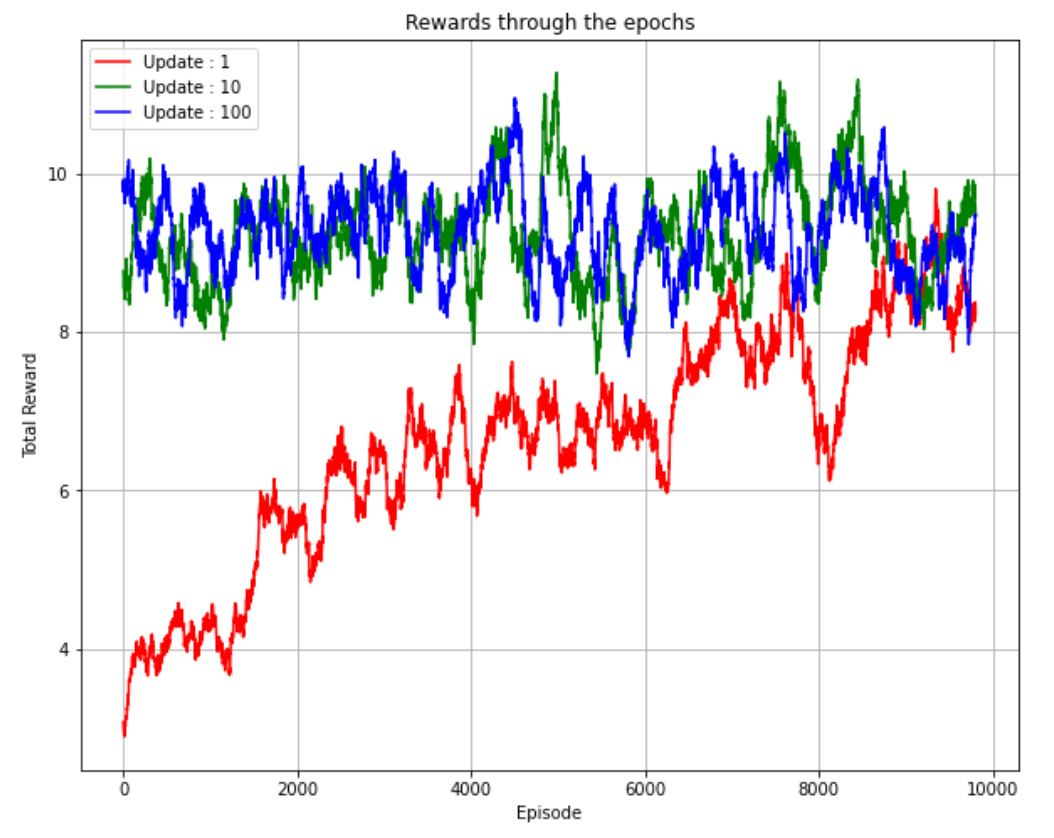
\includegraphics[width=5cm]{img/reward_dq_iter.png} }}%
        \qquad
        \subfloat[Loss]{{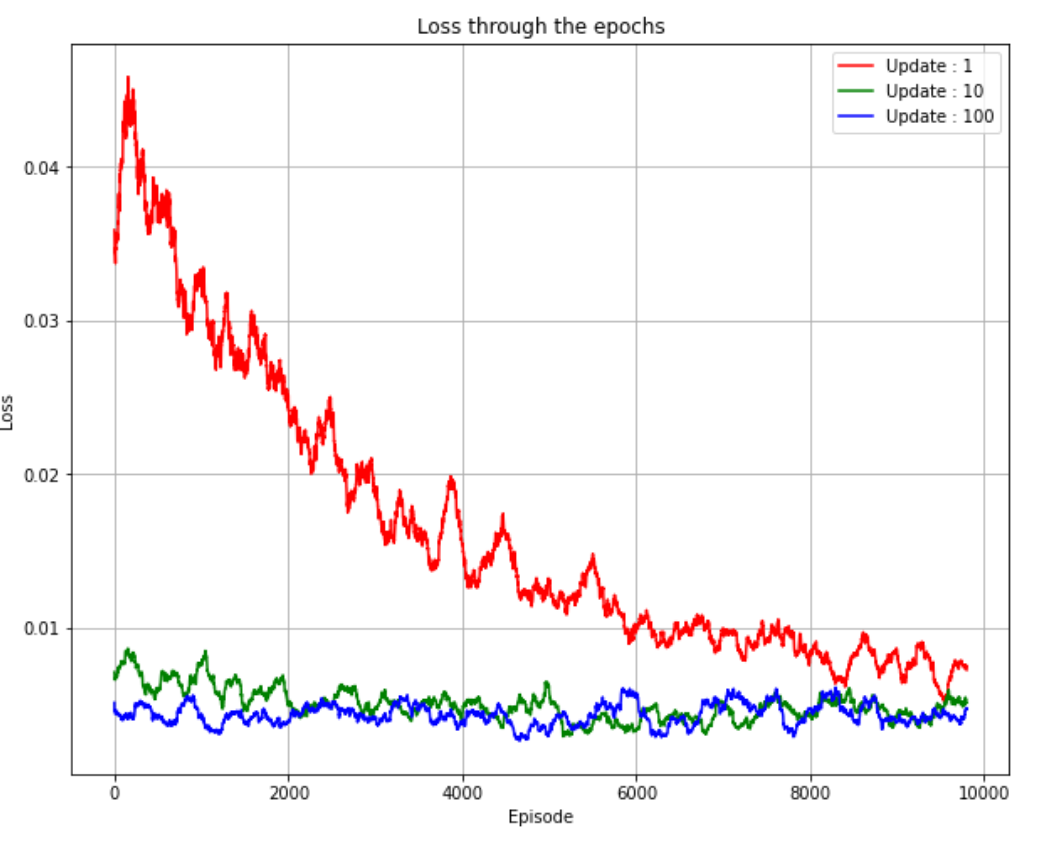
\includegraphics[width=5cm]{img/loss_dq_iter.png} }}%
        \caption{Reward and Loss for different target update with 'multiple' as representation and $\gamma$ = 0, linear model }%
        \label{fig:example}%
        \end{figure}

    We see that for an update C = 1, which is basically the deep Q-learning used before, it converges slowly. The effect of stabilizing the target network leads it to learn quickly. It doesn't seem to have effect on the noise. Furthermore, it has same behaviour for C = 10 and C = 100 (C = 100 corresponds to an update every 10 episodes, because we increment C every time a suggestion is made and the batch size is 10). 

\subsection{Results}
    What we added from the classic Q-learning algorithm is the stability of the target and a different state representation.
    We compare the results only for $\gamma = 0.9$, because it has indeed solved the case $\gamma$ = 0. We also tried with the 'rewards' representation to see if the representation has added something.
    
    \subsubsection{Rewards and Loss}
    We ran the algorithm for 20 000 epochs, with a memory size of 200 and update target C = 50. 
    \begin{figure}[h!]
        \centering
        \subfloat[Rewards]{{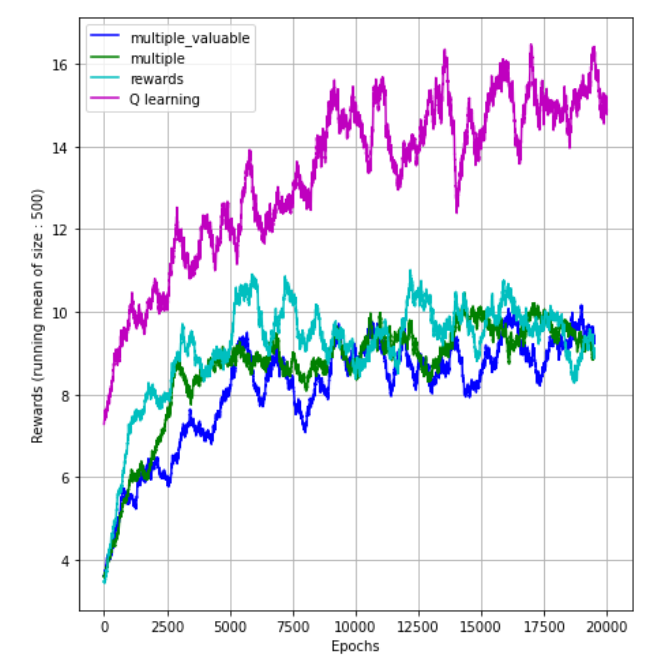
\includegraphics[width=5cm]{img/rewards_20000.png} }}%
        \qquad
        \subfloat[Loss]{{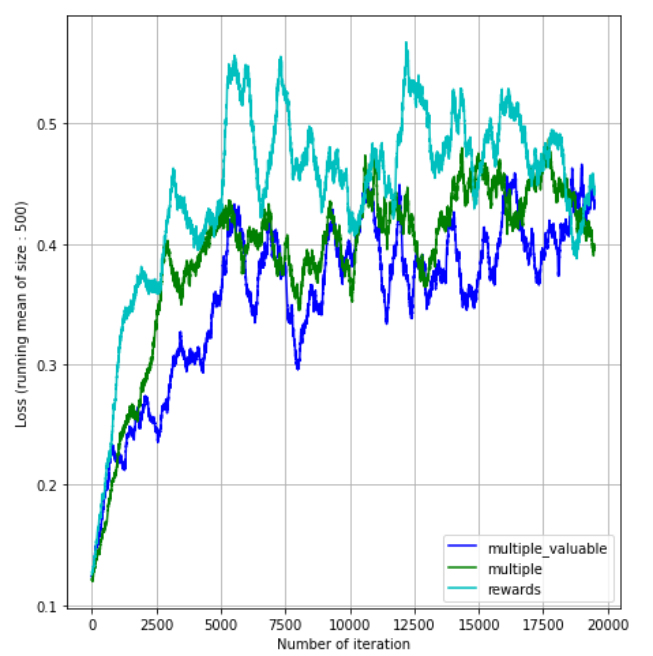
\includegraphics[width=5cm]{img/loss_20000.png} }}%
        \caption{Reward and Loss with double Q-learning for different representation states, $\gamma = 0.9$ and fully connected of size 300 }%
        \label{fig:example}%
        \end{figure}
    
    The Figure 23 shows that it learns better than with the Q-learning algorithm. It achieves a reward of 9, which is almost what we get with $\gamma = 0$. Nevertheless, the loss doesn't have the expected behaviour. It can be explained by the fact that the network has found the relevant actions, but not the accurate values (the expected Q-values with the Q-learning method are around 1.6 and the final values with the double-q learning are around 4.5). \\
    Furthermore, we also notice that the new representations don't bring much information : the rewards representation converge. What is better than before is the target network which is not the same as the prediction. This should be that point that enable the algorithm to converge. \\
    We also notice that the double Q-learning algorithm converges faster than the Q-learning algorithm. 
    
    \subsubsection{Q-table}
    We got the following q-tables for the previous parameters : 
    
     \begin{figure}[h!]
            \centering
            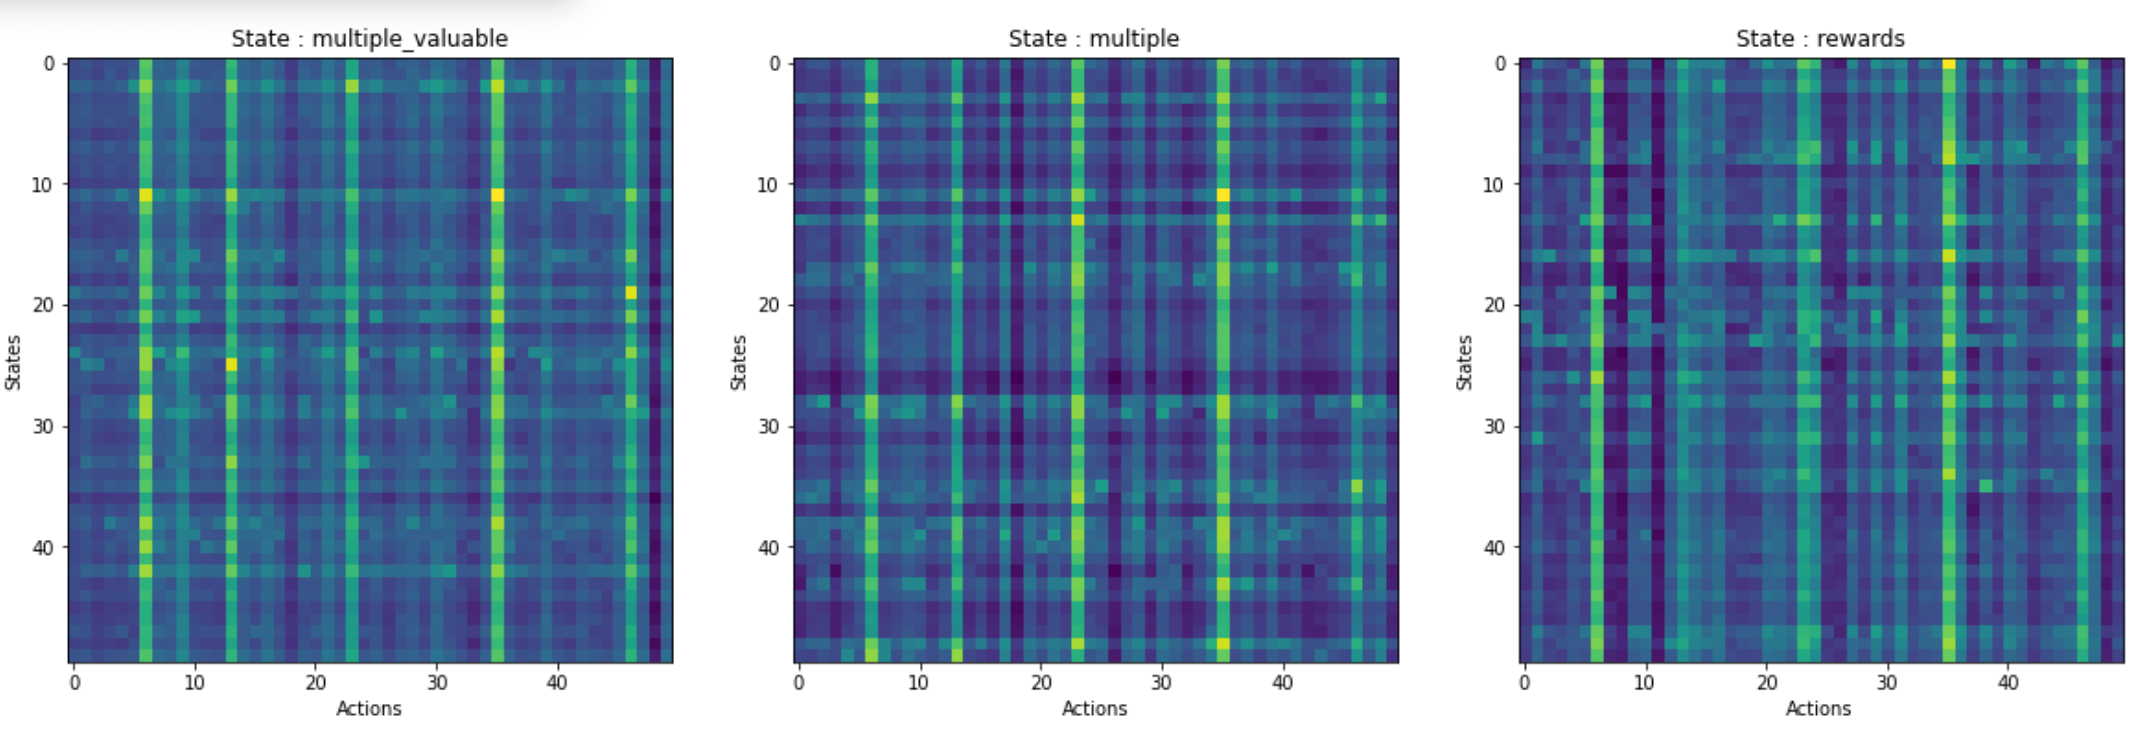
\includegraphics[scale = 0.4]{img/q_tables_20000.png}
            \caption{Q-table for different representation and $\gamma = 0.9$ : multiple valuable, multiple and rewards}
            \label{fig:my_label}
        \end{figure}
    
    It seems that the algorithm has distinguished the cached content, but not all the related items. Furthermore, the values should be very close. This is in fact the case. 
    \newpage
     \begin{figure}[h!]
            \centering
            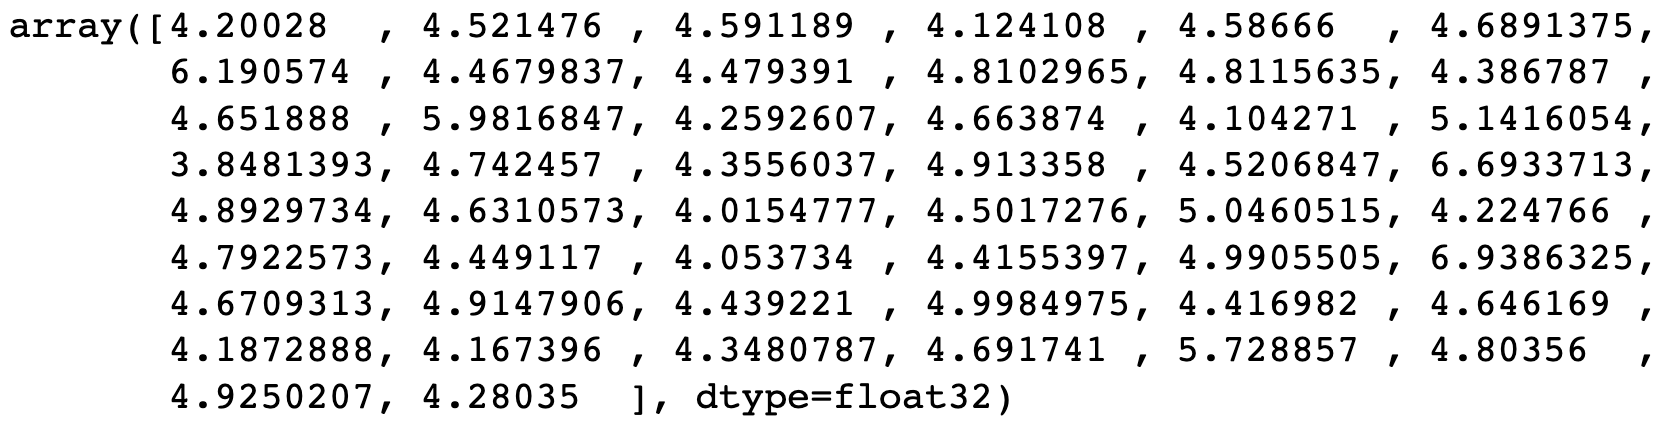
\includegraphics[scale = 0.4]{img/q_table_0.png}
            \caption{Q-table for 'multiple' representation for state 0}
            \label{fig:my_label}
        \end{figure}
    
    It seems that it has stabilised around 4 for the Q-table values (whereas it should be around 1.6 with the q-learning algorithm). This gap can be explained by the state representation which seems still too detailed. 


\section{Conclusion}

We've implemented algorithms that aim to deal with network latency. Indeed, the main goal of this project was to find a trade-off by creating a reinforcement algorithm where an agent (the recommender) had to interact with a user. This user has some preferences (which corresponds to the related items) and can have access easily to few contents of the catalogue. Therefore, with the Q-learning algorithm, the agent can have an idea of what is good to recommend or not by trying it. Nevertheless, such approach is limited because a user won't consume every content of the catalogue. To avoid this, we implemented function approximation algorithms like deep Q-learning or double Q-learning. The purpose of these methods is to find similarity on contents in order to infer the rewards, and avoiding exploring each content. Nevertheless, our implementation doesn't seem to have reach this approximation : this is more of a tabular method.  This can be limited by the representation of our states, which has been the main limitations for the success of the approximation.





\begin{thebibliography}{99}


\bibitem{Giannakas, Theodoros and Sermpezis, Pavlos and Spyropoulos, Thrasyvoulos} 

Giannakas, Theodoros and Sermpezis, Pavlos and Spyropoulos, Thrasyvoulos, 2018.
\textit{Show me the Cache: Optimizing Cache-Friendly Recommendations for Sequential Content Access}


\bibitem{Richard S. Sutton and Andrew G. Barto} 

Richard S. Sutton and Andrew G. Barto, 2018.
\textit{Reinforcement Learning: An Introduction, second edition}

\bibitem{Pytorch} 
Pytorch tutorials on reinforcement learning
\\\texttt{https://pytorch.org/tutorials/intermediate/reinforcement\_q\_learning.html}

\bibitem{Pong from Pixels} 
Deep Reinforcement Learning: Pong from Pixels
\\\texttt{https://karpathy.github.io/2016/05/31/rl/}

\bibitem{A Hands-On Introduction to Deep Q-Learning using OpenAI Gym in Python} 
A Hands-On Introduction to Deep Q-Learning using OpenAI Gym in Python
\\\texttt{https://www.analyticsvidhya.com/blog/2019/04/introduction-deep-q-learning-python/}

\bibitem{An introduction to Deep Q-Learning: let’s play Doom} 
An introduction to Deep Q-Learning: let’s play Doom
\\\texttt{https://www.freecodecamp.org/news/an-introduction-to-deep-q-learning-lets-play-doom-54d02d8017d8/}

\bibitem{Getting Started with Gym} 
Getting Started with Gym
\\\texttt{https://gym.openai.com/docs/}









\end{thebibliography}











\end{document}